% Unofficial Umich Poster template.
% A fork of the MSU template https://www.overleaf.com/latex/templates/an-unofficial-poster-template-for-michigan-state-university/wnymbgpxnnwd
% which is a fork of https://www.overleaf.com/latex/templates/an-unofficial-poster-template-for-new-york-university/krgqtqmzdqhg
% which is a fork of https://github.com/anishathalye/gemini
% also refer to https://github.com/k4rtik/uchicago-poster



\documentclass[final]{beamer}

% ====================
% Packages
% ====================

\usepackage[T1]{fontenc}
\usepackage[utf8]{inputenc}
\usepackage{lmodern}
\usepackage{threeparttable}
\usepackage{multirow}
\usepackage[size=custom, width=121.92, height=91.44, scale=1.2]{beamerposter}
\usetheme{gemini}
% Custom Harvard Crimson color theme
\definecolor{harvardcrimson}{RGB}{165, 28, 48}
\definecolor{harvardgray}{RGB}{80, 79, 79}
\usepackage{bm}
\usepackage{multicol}
% \usepackage[style=authoryear]{biblatex}
% \addbibresource{poster.bib}

\setbeamercolor{palette primary}{bg=harvardcrimson,fg=white}
\setbeamercolor{palette secondary}{bg=harvardcrimson,fg=white}
\setbeamercolor{palette tertiary}{bg=harvardcrimson,fg=white}
\setbeamercolor{palette quaternary}{bg=harvardcrimson,fg=white}
\setbeamercolor{structure}{fg=harvardcrimson}
\setbeamercolor{title}{fg=white,bg=harvardcrimson}
\setbeamercolor{headline}{fg=white,bg=harvardcrimson}
\setbeamercolor{footline}{fg=white,bg=harvardcrimson}
% Normal blocks — black headings, white body
\setbeamercolor{block title}{fg=black,bg=white}
\setbeamercolor{block body}{fg=black,bg=white}

% Alertblocks — black headings, tinted body to distinguish
\setbeamercolor{block alerted title}{fg=black,bg=harvardcrimson!6}
\setbeamercolor{block alerted body}{fg=black,bg=harvardcrimson!6}

\newcommand{\blockrule}{\vspace{-1.5em}\textcolor{harvardcrimson}{\rule{\linewidth}{1.2pt}}\vspace{-0.2em}}

\usepackage{graphicx}
\usepackage{booktabs}
\usepackage{tikz}
\usepackage{pgfplots}
\pgfplotsset{compat=1.14}
\usepackage{anyfontsize}
\usepackage{qrcode}   % <-- moved here, after pgfplots
\usepackage{dsfont}
\usepackage{float}

% ====================
% Lengths
% ====================

% If you have N columns, choose \sepwidth and \colwidth such that
% (N+1)*\sepwidth + N*\colwidth = \paperwidth
\newlength{\sepwidth}
\newlength{\colwidth}
\setlength{\sepwidth}{0.025\paperwidth}
\setlength{\colwidth}{0.3\paperwidth}

\newcommand{\separatorcolumn}{\begin{column}{\sepwidth}\end{column}}

% ====================
% Title
% ====================

\title{Trajectory-Aware Prompt Optimization for AI Agents}

\author{Michael Culver \and Jinyu Han \and Jerry Kim \and Matthew Michel \and Kaylee Vo}

\institute[shortinst]{Harvard Extension School - Harvard University}


% ====================
% Footer (optional)
% ====================

\footercontent{
  \href{https://github.com}{Github: https://github.com/Trajectory-Lab/} \hfill
Agentic AI Summit 2026 Poster Session \hfill
  \href{mailto:kav418@g.harvard.edu}{kav418@g.harvard.edu}}
% (can be left out to remove footer)

% ====================
% Logo (optional)
% ====================

% use this to include logos on the left and/or right side of the header:
% Left: institution
 % \logoright{
\includegraphics[height=8cm]{logos/seas_logo.png}}
% Right: funding agencies and other affilations 
%\logoright{\includegraphics[height=7cm]{logos/NSF.eps}}
% ====================
% Body
% ====================

% use this to include logos on the left and/or right side of the header:
% Left: institution
\logoleft{\qrcode[height=8cm]{https://kayleeisokay.github.io/}}
% Right: funding agencies and other affilations 
\logoright{
\includegraphics[height=8cm]{logos/ExtensionFlag_2.png}}

\begin{document}

\begin{frame}[t]
\begin{columns}[t]
\separatorcolumn

%======================================================================
% COLUMN 1
%======================================================================
\begin{column}{\colwidth}

  \begin{block}{Introduction}
  \blockrule

    Prompt optimization offers a \textbf{gradient-free} alternative to reinforcement learning (RL) for improving LLM agents. Instead of updating model weights, our approach optimizes the instructions an agent conditions on, leaving model weights frozen. We use \textbf{GEPA}, a reflective prompt optimizer, applied to \textbf{DSPy} agent modules operating inside \textbf{GEM}, a standardized gym environment with per-turn dense rewards and published RL baselines \cite{gem2025}.

    \textbf{Research question}: How much of RL's performance can token-space prompt optimization recover, and at what infrastructure cost?

  \end{block}
    \vspace{-0.5em}
  \begin{block}{Motivation}
    \blockrule
    
    Training agentic LLMs with RL requires gradient updates, rollout infrastructure, and substantial compute, which is costly. Developing \textbf{less costly} approaches to agent optimization allows smaller operations access to agent-based technologies. 

    We evaluate our approach against two reference points: (1) the model's own \textbf{unoptimized prompt}, and (2) \textbf{published GEM RL results}.
  \end{block}
  \begin{alertblock}{Contributions}
  \blockrule
    \begin{enumerate}
      \item A \textbf{GEM--DSPy adapter} bridging RL-designed gym environments with token-space prompt optimization.
      \item A \textbf{trajectory-aware composite fitness function} combining discounted return, loop-detection penalty, and step/call-efficiency bonuses.
      \item A full \textbf{baseline-vs-optimized benchmark} across four agentic environments, six model families, and three seed replications.
    \end{enumerate}
  \end{alertblock}
    \vspace{-1em}
    
  \begin{block}{Method}
  \blockrule
  
    Agents are LLMs embedded in the DSPy module, following the ReAct pattern \cite{react2023}. GEPA mutates only the instruction text. \textbf{Environments}: HotpotQA (multi-hop QA, with/without tool) and Orz57K (math reasoning, with/without tool).

    \textbf{Models:}
        \vspace{-0.5em}
        \begin{multicols}{2}
        \begin{itemize}
            \item Qwen3-1.7B-Base
            \item Qwen3-4B-Base
            \item Llama-3.1-8B-Instruct
            \item Gemma-3-4B-IT
            \item Mistral-7B-Instruct
            \item Nemotron-Nano-9B
        \end{itemize}
        \end{multicols}

\textbf{Training Loop: Iterative Prompt Refinement}

\begin{enumerate}
    \item \textbf{Mutate.} A reflection language model rewrites the current system prompt. The solver is the task-model-driven agent, wrapped as a DSPy module. Behavior is entirely parameterized by the prompt GEPA mutates.

    \item \textbf{Rollout.} For each training example:
    \begin{itemize}
        \item The solver extracts the current instructions and uses them as its system prompt
        \item A fresh episode is initialized in the environment (GEM), producing an initial observation
        \item The solver interacts with GEM step by step: it observes the state, selects an action, the environment updates and returns a new observation, reward, and completion signal, and each step is logged
        \item The episode ends if a terminal state is reached
        \item The result is a complete trajectory log of the episode
    \end{itemize}

    \item \textbf{Score.} The fitness metric evaluates the trajectory. The composite score is normalized and accompanied by a human-readable breakdown explaining \emph{why} the trajectory received that score.

    \item \textbf{Update.} Rather than keeping only the single best prompt, the optimizer maintains a \emph{Pareto frontier} of promising prompt candidates (total of 12 candidates). The reflection model reads the score breakdown as feedback to propose the next round of prompt mutations.
\end{enumerate}


  \end{block}

\end{column}

\separatorcolumn

%======================================================================
% COLUMN 2 — RESULTS
%======================================================================
\begin{column}{\colwidth}
    \begin{alertblock}{Fitness Function}
    \blockrule
    
    The fitness $F(\tau)$ is implemented as a weighted composite of four terms,
   
    \begin{equation}
    \label{eq:fitness_composite}
    F(\tau) \;=\; \tilde{F}_{\mathrm{ret}}(\tau) \;+\; w_{\mathrm{loop}}\, F_{\mathrm{loop}}(\tau) \;+\; w_{\mathrm{step}}\, F_{\mathrm{step}}(\tau) \;+\; w_{\mathrm{call}}\, F_{\mathrm{call}}(\tau).
    \end{equation}

1. Normalized Discounted Return:
    \begin{equation}
    \label{eq:fitness_return}
        \tilde{F}_{\mathrm{ret}}(\tau) \;=\; \frac{R_T\sum_{t=0}^{T-1}\gamma^{T-1-t} \;+\; \lambda\sum_{t=0}^{T-1} r_{t+1}}{\sum_{t=0}^{T-1}\gamma^{T-1-t} \;+\; \lambda\, T}, \qquad R_T \;=\; \mathds{1}[r_T > 0].
    \end{equation}

    \begin{itemize}
        \item Discount runs in \emph{reverse time}: the exponent $T{-}1{-}t$ assigns full weight $\gamma^{0}=1$ to the final step and discounts earlier steps.
        \item Gated by $R_T$, credit from the discounted-return component ($\Sigma\gamma^{T-1-t}$) accrues only when the trajectory terminates with positive final reward, while the auxiliary per-step term ($\lambda\Sigma r_{t+1}$) is added unconditionally.
    \end{itemize}

2. Loop-detection Penalty:

    \begin{equation}
    \label{eq:fitness_loop}
    F_{\mathrm{loop}}(\tau) \;=\; -\,\frac{1}{T-1}\sum_{t=1}^{T-1}\mathds{1}\!\left[a_t \in \{a_s : \max(0, t-W) \le s < t\}\right].
    \end{equation}
    \begin{itemize}
        \item Returns a value in $[-1,0]$ and discourages identical-action repetition within a sliding window. Window size $W$ is a hyperparameter, set to 3.
    \end{itemize}
    

3. Step-efficiency Bonus:
        \begin{equation}
        \label{eq:fitness_step}
        F_{\mathrm{step}}(\tau) \;=\; R_T\cdot\max\!\left(0,\; 1 - \frac{T}{T_{\max}}\right), \qquad T_{\max}=50.
        \end{equation}
        \begin{itemize}
            \item For trajectories with $T<T_{max}$, the agent receives a bonus reward.
        \end{itemize}

4. Call-efficiency Bonus:
    \begin{equation}
    \label{eq:fitness_call}
    F_{\mathrm{call}}(\tau) \;=\; R_T\cdot\max\!\left(0,\; 1 - \frac{\sum_{t=0}^{T-1}\big(|c^{\mathrm{LLM}}_t|+|c^{\mathrm{tool}}_t|\big)}{T_{\max}\cdot B}\right), \qquad B=8.
    \end{equation}
    \begin{itemize}
        \item Rewards successful trajectories whose total per-step LLM and tool-call counts $|c^{\mathrm{LLM}}_t|+|c^{\mathrm{tool}}_t|$ remain well within the budget $T_{\max}\cdot B$.
    \end{itemize}
    \end{alertblock}

 \vspace{-1.5em}
\begin{block}{Example of Prompt Evolution}
    \blockrule
    \begin{figure}
      \centering
      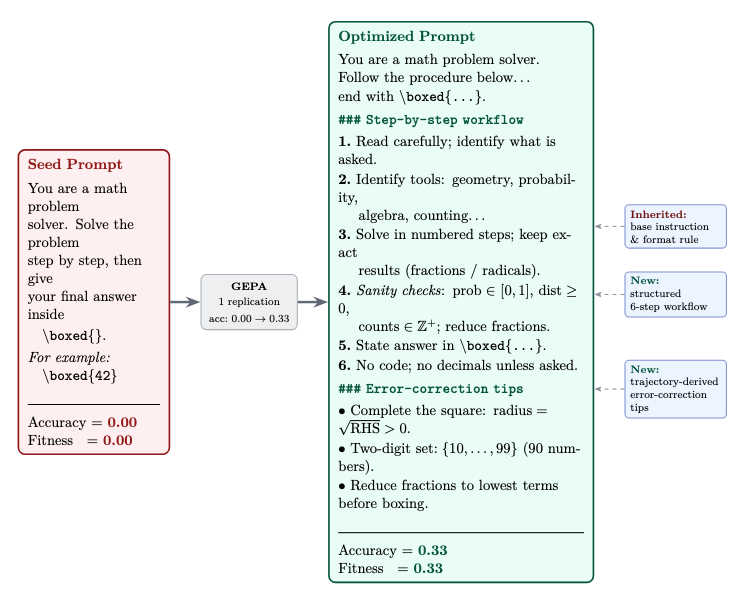
\includegraphics[width=0.75\textwidth]{plots/trajectory/prompt_evolution.png}
      \caption{Example of prompt evolution in one GEPA replication on a mathematics benchmark.}
    \end{figure}
\end{block}
  
    

\end{column}

\separatorcolumn

%======================================================================
% COLUMN 3 — EQUIVALENCE, COST, LIMITATIONS
%======================================================================
\begin{column}{\colwidth}
    \begin{alertblock}{Experiment Results}
    \blockrule
    
    \begin{figure}[H]
    \centering
    \begin{tikzpicture}
    \begin{axis}[
        width=0.75\linewidth,
        height=11cm,
        ybar,
        bar width=45pt,
        ymin=0,
        ymax=0.5,
        title={HotpotQA with Search Tool},
        title style={font=\large},
        ylabel={Task Success Rate},
        symbolic x coords={Qwen1.7B,Qwen4B,Llama,Gemma,Mistral,Nemotron},
        xtick=data,
        enlarge x limits=0.15,
        ymajorgrids=true,
        grid style={dotted},
        tick align=outside,
        clip=false,
        x tick label style={rotate=30, anchor=east, font=\footnotesize, yshift=-16pt},
        y tick label style={font=\footnotesize},
        label style={font=\normalsize},
        legend pos=north west,
        legend style={legend columns=1, font=\footnotesize, fill=white, fill opacity=0.85, draw=gray},
    ]
    \addplot coordinates {(Qwen1.7B,0.001) (Qwen4B,0.027) (Llama,0.033) (Gemma,0.095) (Mistral,0.022) (Nemotron,0.095)};
    \addlegendentry{Baseline}
    \addplot coordinates {(Qwen1.7B, 0.049) (Qwen4B,0.043) (Llama,0.221) (Gemma,0.289) (Mistral,0.155) (Nemotron,0.101)};
    \addlegendentry{Optimized}
    \draw [black, dashed, thick]
        ({rel axis cs:0,0}|-{axis cs:Qwen1.7B,0.432}) --
        ({rel axis cs:1,0}|-{axis cs:Qwen1.7B,0.432});
    \node [anchor=east, font=\footnotesize, fill=white, inner sep=2pt]
        at (axis cs:Nemotron,0.432) {RL ref = 0.432};
    \addlegendimage{legend image code/.code={\draw[black,dashed,thick] (0mm,0mm) -- (6mm,0mm);}}
    \addlegendentry{RL Reference}
    \end{axis}
    \end{tikzpicture}
    \vspace{-1.5em}
    \caption{HotpotQA with tool: mean baseline and optimized values vs.\ RL reference.}
    \label{fig:hotpotqa_tool_chart}
\end{figure}
\vspace{-0.5em}
\begin{figure}[H]
    \centering
    \begin{tikzpicture}
    \begin{axis}[
        width=0.75\linewidth,
        height=11cm,
        ybar,
        bar width=45pt,
        ymin=0,
        ymax=0.5,
        title={HotpotQA without Search Tool},
        title style={font=\large},
        ylabel={Task Success Rate},
        symbolic x coords={Qwen1.7B,Qwen4B,Llama,Gemma,Mistral,Nemotron},
        xtick=data,
        enlarge x limits=0.15,
        ymajorgrids=true,
        grid style={dotted},
        tick align=outside,
        clip=false,
        x tick label style={rotate=30, anchor=east, font=\footnotesize, yshift=-18pt},
        y tick label style={font=\footnotesize},
        label style={font=\normalsize},
        legend pos=north west,
        legend style={legend columns=1, font=\footnotesize, fill=white, fill opacity=0.85, draw=gray},
    ]
    \addplot coordinates {(Qwen1.7B,0.044) (Qwen4B,0.057) (Llama,0.340) (Gemma,0.122) (Mistral,0.098) (Nemotron,0.123)};
    \addlegendentry{Baseline}
    \addplot coordinates {(Qwen1.7B,0.119) (Qwen4B,0.168) (Llama,0.333) (Gemma,0.245) (Mistral,0.196) (Nemotron,0.186)};
    \addlegendentry{Optimized}
    \draw [black, dashed, thick]
        ({rel axis cs:0,0}|-{axis cs:Qwen1.7B,0.211}) --
        ({rel axis cs:1,0}|-{axis cs:Qwen1.7B,0.211});
    \node [anchor=east, font=\footnotesize, fill=white, inner sep=2pt, yshift=14pt]
        at (axis cs:Nemotron,0.211) {RL ref = 0.211};
    \addlegendimage{legend image code/.code={\draw[black,dashed,thick] (0mm,0mm) -- (6mm,0mm);}}
    \addlegendentry{RL Reference}
    \end{axis}
    \end{tikzpicture}
    \vspace{-1.5em}
    \caption{HotpotQA without tool: mean baseline and optimized values vs.\ RL reference.}
    \label{fig:hotpotqa_notool_chart}
\end{figure}
    The results of our approach \textbf{do not match the performance of RL-based methods} given in the GEM paper \cite{gem2025}. We observe improvements over the baseline of simply using unoptimized prompts. Only Gemma without tooling provides a performance boost equivalent to the RL-based methods.


  \end{alertblock}

  
    \vspace{-1.4em}
  \begin{block}{Resource Use \& Cost}
    \blockrule
    
    Mean per-run cost across completed cells: \textbf{\$0.35--\$4.45}. No-tool settings are consistently cheaper than with tooling. All runs are cheaper than GPU-based RL training. For HotpotQA-notool, Gemma's run gained 12.3 percentage points (pp) of accuracy at a cost of \$0.346, giving an efficiency of 35.5 pp/\$.
    \vspace{-1em}
    \begin{table}[H]
    \centering
    % \caption{Primary Comparison Cells (Gemma and Llama)}
    \label{tab:cost_efficiency_table}
    \small
    \setlength{\tabcolsep}{4pt}
    \resizebox{\textwidth}{!}{%
    \begin{tabular}{llrrrr}
    \toprule
    \textbf{Environment} & \textbf{Model} & \textbf{Base} & \textbf{Opt.} & \textbf{Cost} & \textbf{Efficiency (pp/\$)} \\
    \midrule
    hotpotqa-notool & Gemma-3-4B-IT & 0.122 & 0.245 & \$0.346 & 35.5 \\
    hotpotqa-notool & Llama-3.1-8B-Instruct & 0.340 & 0.333 & \$1.100 & $-$0.6 \\
    hotpotqa-tool & Gemma-3-4B-IT & 0.095 & 0.289 & \$0.737 & 26.3 \\
    hotpotqa-tool & Llama-3.1-8B-Instruct & 0.033 & 0.221 & \$4.451 & 4.2 \\
    \bottomrule
    \end{tabular}}
    \normalsize
    \end{table}
  \end{block}
    \vspace{-1em}

    \begin{block}{Future Work}
    \blockrule
    \begin{enumerate}
        \item Isolate the contribution of specific fitness components through ablation studies to distinguish whether the gains arise primarily from dense reward use, loop penalties, efficiency terms, or the reflective mutation process itself.
        \item Investigate the boundary between policy and capability shaping more directly. 
    \end{enumerate}
    \end{block}
    
    \vspace{-1.4em}
  \begin{block}{References}
    \blockrule
    \nocite{*}
    \footnotesize{\bibliographystyle{plain}\bibliography{poster}}
  \end{block}

\end{column}

\separatorcolumn
\end{columns}
\end{frame}

\end{document}